\section{Třetí verze}
\label{E3-vyvoj}

Třetí verze (E3) do značné míry vycházela z předchozí verze a dále na ní stavěla. Asi nejvýraznější změna bylo navýšení počtu 
LED z dvanácti (hodiny) na šedesát (minuty), což pochopitelně znamenalo i zvětšení kruhu. Na desku se ale přidaly i nové funkcionality,
a~to gyroskop,\footnote{pro možnost znalosti náklonu zařízení} akcelerometr,\footnote{pro znalost směru a~velikosti zrychlování} magnetický kompas,\footnote{pro určení světových
stran} RTC\footnote{Real Time Clock, hodiny reálného času, pro znalost přesného času} a GPS.\footnote{pro možnost určení svojí polohy}
Také jsem použil, po vzoru mechanického trezoru, rotační západku, což znamenalo, že na stejný trezor se daly použít jak mechanické tak 
elektronické dveře.

Z důvodů použití převodů pro otáčení rotační západky byly nově také použité díly tištěné na 3D tiskárně. 

Tato verze měla dvě varianty, které se lišily motorem.
Motor vpravo na obrázku \obr{fig:E3-motory} byl použit na dřívější verzi a později jsem jej vyměnil za motor nalevo, díky čemuž jsem dveře mohl udělat tenčí. %todo přečíst 
\begin{figure}[htbp]
    \centering
    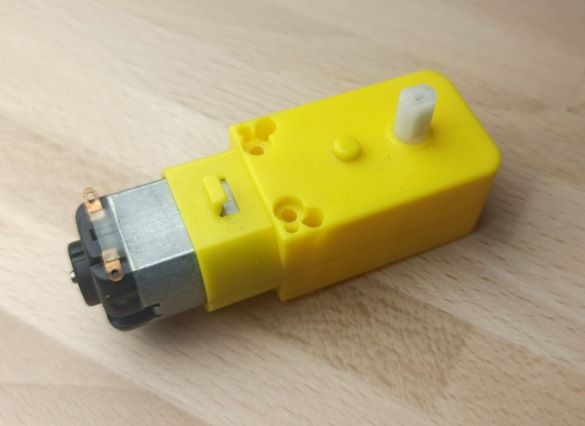
\includegraphics[height=140pt]{kapitoly/obrazky/E3/motory/zluty_motor.jpg}
    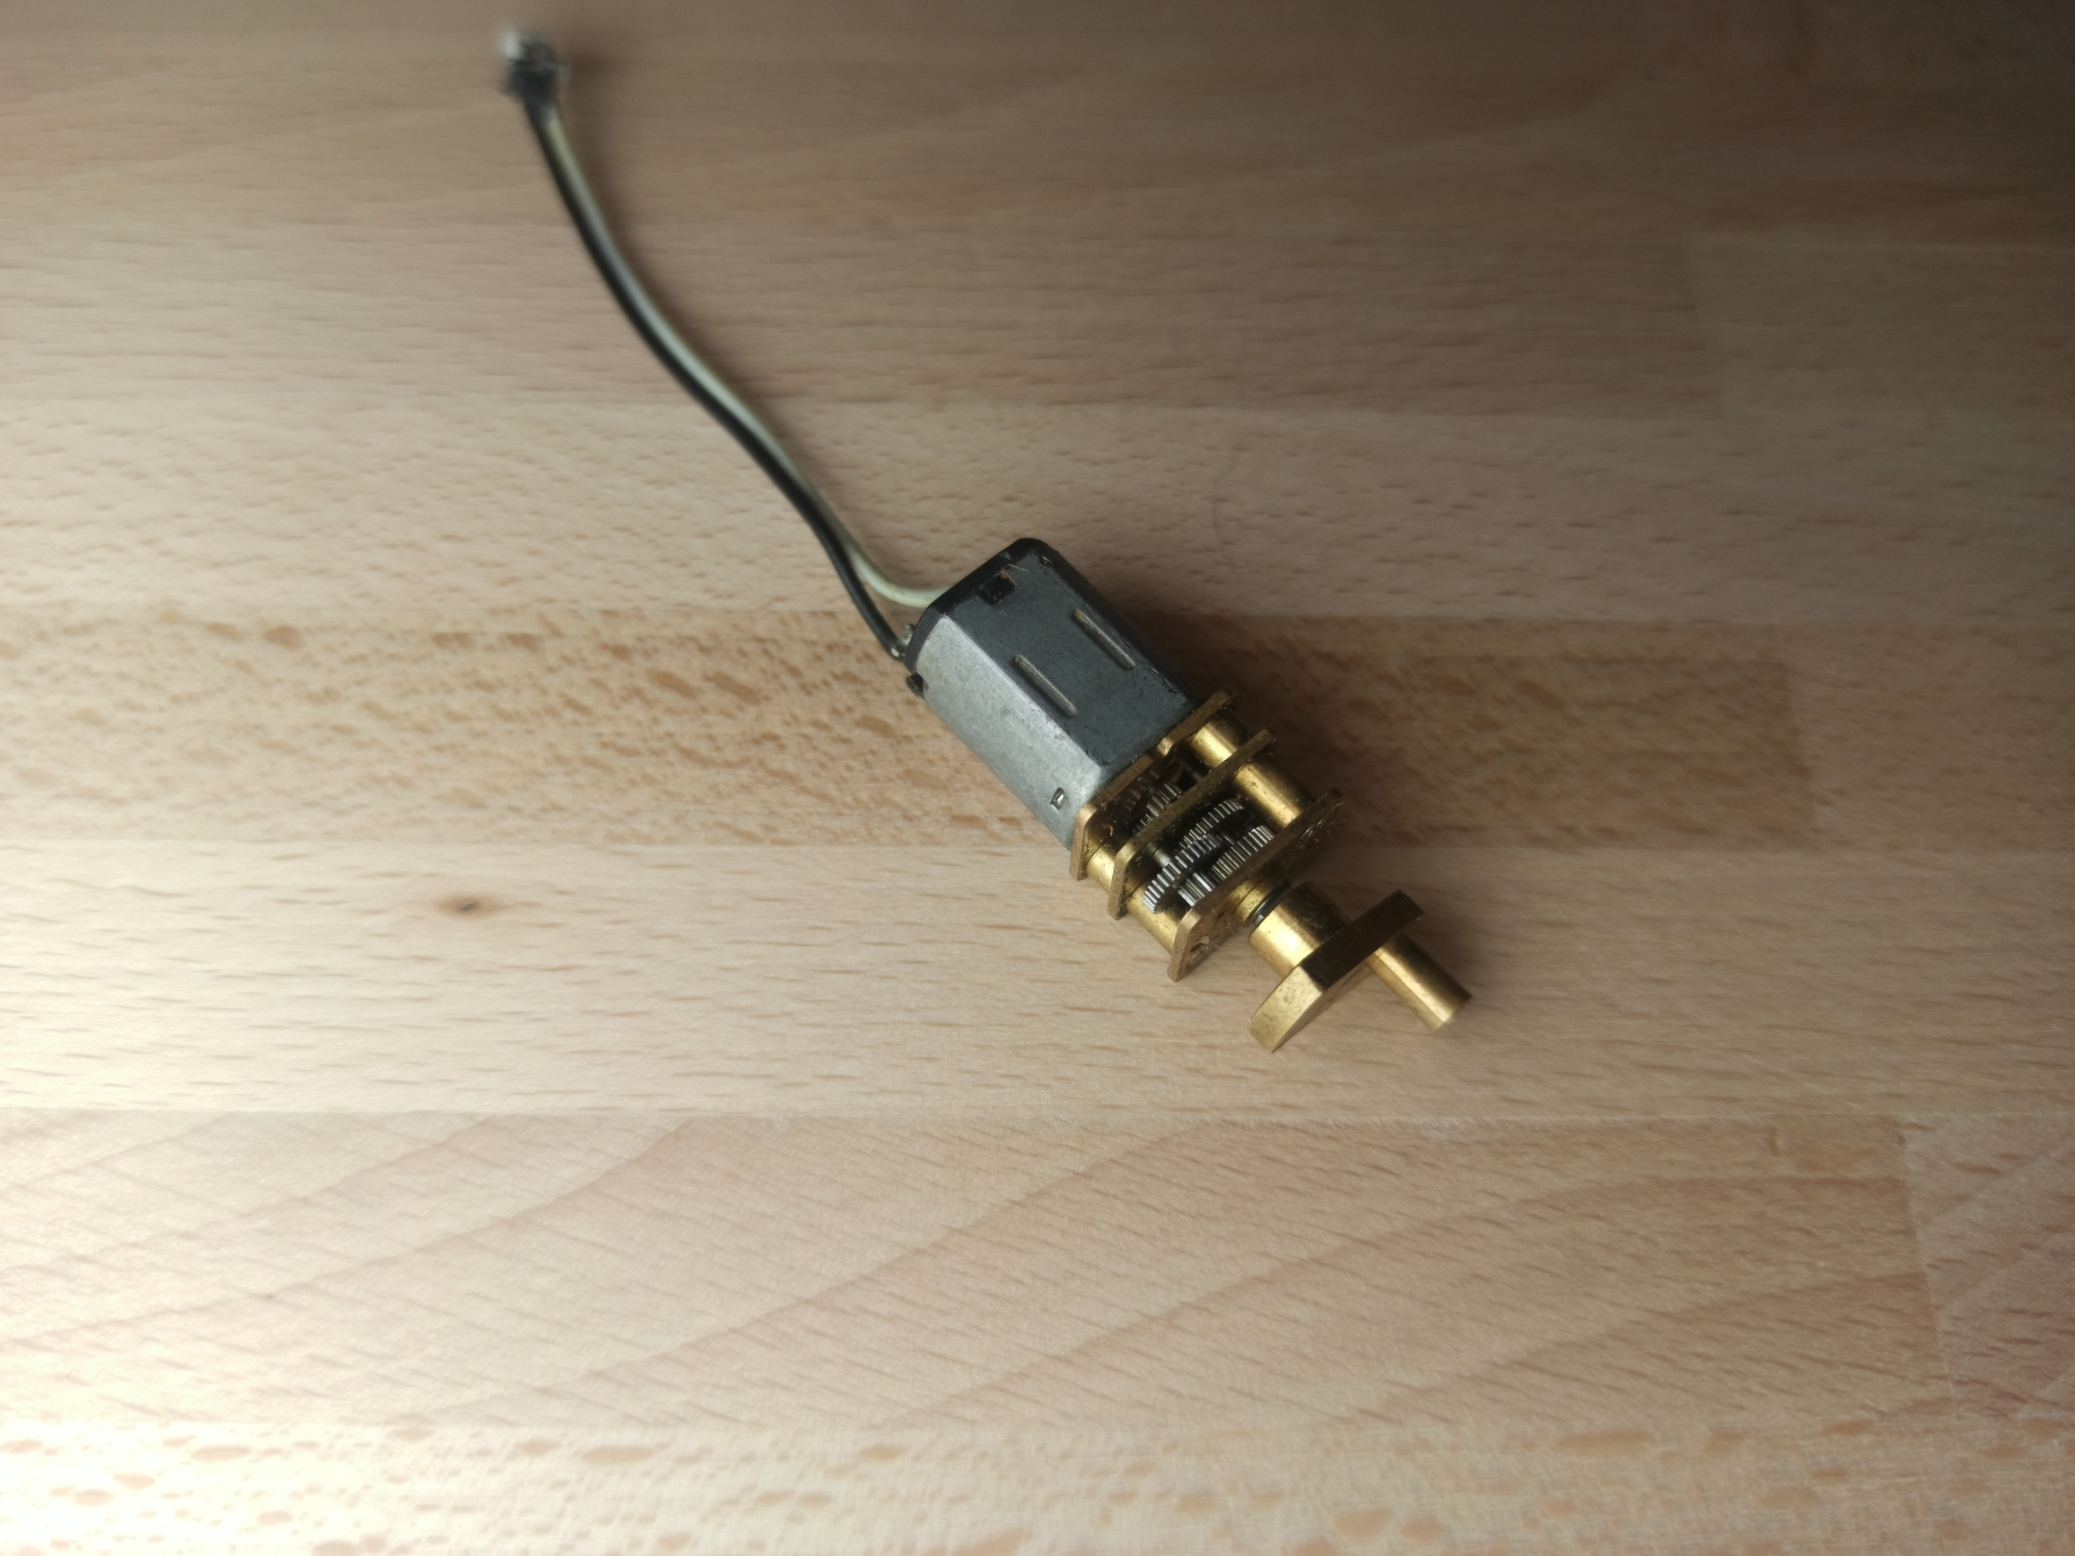
\includegraphics[height=140pt]{kapitoly/obrazky/E3/motory/hodinovyStrojek.jpg}
    \caption{Fotografie obou testovaných motorů} 
    \label{fig:E3-motory}
\end{figure}

\newpage